% !TeX root = RJwrapper.tex
\title{PINstimation: An R Package for Estimating Probability of Informed Trading Models}


\author{by Montasser Ghachem and Oguz Ersan}

\maketitle

\abstract{%
The purpose of this paper is to introduce the R package \href{https://CRAN.R-project.org/package=PINstimation}{PINstimation}. The package is designed for fast and accurate estimation of the probability of informed trading models through the implementation of well-established estimation methods. The models covered are the original PIN model (Easley and O'Hara 1992; Easley et al. 1996), the multilayer PIN model (Ersan 2016), the adjusted PIN model (Duarte and Young 2009), and the volume- synchronized PIN (Easley, De Prado, and O'Hara 2011; Easley, López De Prado, and O'Hara 2012). These core functionalities of the package are supplemented with utilities for data simulation, aggregation and classification tools. In addition to a detailed overview of the package functions, we provide a brief theoretical review of the main methods implemented in the package. Further, we provide examples of use of the package on trade-level data for 58 Swedish stocks, and report straightforward, comparative and intriguing findings on informed trading. These examples aim to highlight the capabilities of the package in tackling relevant research questions and illustrate the wide usage possibilities of PINstimation for both academics and practitioners.
}

\section{Introduction}

Informed trading indicates the presence of information asymmetry in a given market, and is usually attributed to trading with better-quality information and/or more sophisticated tools for analyzing available information \citep[see][]{Ahn2008Informed}. Given its impact on prices and liquidity, researchers have dedicated considerable effort to the measurement of informed trading, and to the characterization of its relevant aspects \citep{Berkman2014Informed,Chang2014dynamic, Bongaerts2014Cross-Sectional,Hsieh2014Informed,Yin2015Hidden, Guo2016Better}. The growth in informed trading measures has been made possible thanks to the availability of rich datasets, and as a response to the continuously evolving nature of trading in financial markets. 

Despite the plethora of alternative and more recent measures, "fundamental" measures developed by the pioneering works are still widely used in academic research. Some prominent measures include: relative trade informativeness measure \citep{Hasbrouck1991Measuring}, percentage-price-impact measure \citep{Huang1996Dealer}, adverse selection component \citep{Huang1997components} and the adverse information parameter \citep{Madhavan1997Why}. Above the rest, the probability of informed trading \citep[PIN;][]{easley1992time, easley1996liquidity} has probably been the most widely used measure of informed trading in the literature. Easley and O'Hara, beginning with their foundational work in 1987 and continuing through subsequent studies in the 1990s and 2000s, developed, tested and refined the PIN measure to quantify informed trading in financial markets.
A major factor behind the persistent wide use (prominence) of the PIN model lies in the branch of studies addressing the limitations of the model, remedying to the challenges of its estimation; and extending the original model. Due to the rapid evolution of trading in financial markets, the estimation of the original PIN model has become vulnerable to errors; and the model – and its assumptions – as it was first suggested has faced difficulties in matching the real world. 
Over the years, many extensions and improvements to the PIN model have been developed, addressing various shortcomings of the original model and estimation challenges. However, because of their more complex theoretical underpinnings and implementation details, most of these models have not been adopted by the wider academic and practitioner audience. To address these issues, the \pkg{PINstimation} package seeks to provide easy and convenient access to these extensions of the PIN model. To this end, the package is designed in a compact structure allowing users to directly obtain informed-trading estimates solely by the use of an intraday trading data. The package includes easy-to-use functions, that accurately implement preexisting, and novel remedial solutions to estimation challenges as suggested in the literature. Besides, it provides a rich toolbox for simulating datasets, something that can help researchers conduct robust, and reliable comparative analyses. By the introduction of the package, we hope to contribute to further use of the PIN models in academic research, to improve the validity, and quality of scientific findings within the field, and eventually to heighten the interest of practitioners in these models. 

To our knowledge, there are two packages available for the estimation of PIN models: \strong{pinbasic} \citep{Recktenwald2018pinbasic,recktenwald2019advanced} and \CRANpkg{InfoTrad} \citep{Celik2017InfoTrad,Celik2018InfoTrad}. Both packages have limited scope as they solely focus on the original PIN model \citep{easley1996liquidity}. In addition to scope differences, other motivations for users to shift to \pkg{PINstimation} are that (1) the package \strong{pinbasic} has recently been placed in the archive by CRAN (2) the package \pkg{InfoTrad} in its current version (V.1.2) is not error-free.\footnote{In fact, two of the five functions suffer from implementation errors. The function \code{EA()} implements the algorithm of \cite{Ersan2016unbiased}, but performs the clustering process inaccurately: the days within the information-event cluster are distributed into good-event and bad-event days via a clustering step based on order imbalance rather than the actual step of grouping them into two based on the sign of order imbalance. The function \code{YZ()} of the same package implements the algorithm of \cite{Yan2012improved}. It, however, contains an error in the denominator of the PIN formula. The correct formula should be $\mathrm{PIN} =\alpha \mu /(\alpha \mu +\varepsilon_{b}+\varepsilon_{s})$. This error might impact the results in research papers using the package (See, for instance, Figure 12 in \cite{griffin2021} – very poor performance of PIN estimates using \code{YZ()}). Our comparative tests confirm those observations, as the mean absolute errors in PIN estimates of \pkg{InfoTrad} and \pkg{PINstimation} implementations are $0.02476$, and $0.00014$ respectively for \cite{Yan2012improved}; and $0.00777$  and $0.00014$ respectively for \cite{Ersan2016unbiased}.}

\pkg{PINstimation} contains functions to estimate probability of informed trading (PIN) as introduced by \cite{easley1992time}, and  \cite{easley1996liquidity}. The estimation procedures implemented in these functions help to avoid floating point errors, boundary solutions, and convergence to local maxima. Besides, the package provides a comprehensive treatment of two important extensions of the PIN model. The multilayer probability of informed trading model \citep[MPIN model;][]{ersan2016multilayer}, in contrast to the original PIN model, allows for multiple information types, and assumes that information events cluster in layers with uniform informed trading intensity. Relaxing the assumption of a unique information type allows for a more realistic, and accurate treatment of informed trading. However, it poses, at least, two additional challenges: (1) the larger parameter space of the MPIN model makes it more likely that the maximum likelihood estimate may lie on the parameter boundary, and (2) An accurate determination of the number of information layers is crucial to produce reliable estimations of the probability of informed trading. \pkg{PINstimation} tackles these two issues by including a function to generate strategic\footnote{Strategic initial parameter sets stand in contrast to those obtained through random selection or grid-search methods, as they are derived from the characteristics of the dataset used for the estimation. They are typically limited in number and meticulously selected to cover relevant areas in the parameter space,  ensuring a more accurate and efficient optimization process.} initial parameter sets, and three functions for estimating the number of information layers in datasets. The second extension is the adjusted probability of informed trading model \citep[AdjPIN model;][]{duarte2009why}. This model challenges the assumption that trading is only performed by uninformed liquidity traders and informed traders, and accounts for the possibility of liquidity shocks to both the buy and sell side. \pkg{PINstimation} provides functions to estimate the AdjPIN measure and the PSOS (probability of a symmetric order flow shock), as well as three functions to generate initial sets of parameters for maximum-likelihood estimation. In addition to the standard maximum-likelihood method, the package provides a novel implementation of the estimation of PIN models via the expectation-conditional maximization algorithm. The speed, and accuracy of this algorithm has been recently documented in \cite{ghachem2022maximum}. As for informed trading in high-frequency settings, \pkg{PINstimation} enables users to estimate the volume-synchronized probability of informed trading \citep[VPIN;][]{Easley2011microstructure, Easley2012Flow}. This measure is an adaptation of the PIN measure to the high-frequency trading, and aims to capture the order flow toxicity in a trading data. Finally, the package offers two supporting utilities: (1) a rich simulation toolbox to simulate data according to the assumptions of the different PIN models and, thereby, test the accuracy of estimation algorithms, and (2) a fast implementation of the prominent trade classification algorithms that allow users to generate daily sequences of buyer-initiated, and seller-initiated trades from raw trading level data. Such sequences are to be used later as inputs for the estimations of PIN, MPIN, and AdjPIN models.

The remainder of this paper is organized as follows. Next section provides a brief introduction to the theoretical background of PIN models. Third section presents a detailed description of the package and illustrates its applications through several examples. Fourth section reports and discusses the results of two empirical investigations conducted using the package. The last section concludes with a summary of the package capabilities and a discussion of its potential extensions.

\section{Theoretical background}
\subsection{PIN model}

\cite{easley1992time} developed a model where the change in the order imbalance is associated to the presence of informed trading. The information can be either positive, leading to excess trading on the buy side, or negative, leading to excess trading on the sell side. On days with no information event, there are only uninformed traders in the market. On the days with a good-information (bad-information) event, informed buyers (sellers) join uninformed buyers and sellers to trade on the information. Statistically, \cite{easley1996liquidity} model total trades by a finite Poisson mixture model, where the numbers of buyer-initiated and seller-initiated trades; follow each a Poisson distribution. The likelihood of observing \code{B} buyer-initiated trades (or buys) and \code{S} seller-initiated trades (or sells) on a trading day is stated as:
\begin{equation}
\label{eq:pindaylkd}
\begin{split}
 L\left(B,S|\Theta\right) = \alpha(1-\delta)e^{-\left(\mu +\varepsilon_{b}\right)}\tfrac{\left(\mu +\varepsilon_{b}\right)^{B}}{B!}e^{-\varepsilon_{s}}\tfrac{\varepsilon_{s}^{S}}{S!}+\alpha \delta e^{-\varepsilon_{b}}\tfrac{\varepsilon_{b}^{B}}{B!}e^{-\left(\mu +\varepsilon_{s}\right)}\tfrac{\left(\mu +\varepsilon_{s}\right)^{S}}{S!}+\left(1-\alpha\right)e^{-\varepsilon_{b}}\tfrac{\varepsilon_{b}^{B}}{B!}e^{-\varepsilon_{s}}\tfrac{\varepsilon_{s}^{S}}{S!} 
\end{split}
\end{equation}
where \(\Theta  =\left(\alpha , \delta ,\mu ,\varepsilon_{b},\varepsilon_{s}\right)\) is the set of parameters to be estimated: \(\alpha\) is the probability of occurrence of information events, \(\delta\) is the conditional probability that the information event is a bad event, \(\mu\) is the informed trading intensity, and \( \varepsilon_{b}\) and \( \varepsilon_{s}\) are uninformed trading intensities on the buy and sell sides, respectively. For a time period of \code{N} days, the joint likelihood of observing a set of daily buys and sells, \( M =\left(B_{i}, S_{i}\right)_{i = 1}^{N}\) is presented as:

\begin{equation}
\label{eq:pinlkd}
\mathcal{L}\left(M|\Theta\right) = \prod_{i = 1}^{N}L\left(B_{i}, S_{i}|\Theta\right) 
\end{equation}

Typically, the estimation of the five parameters is performed via maximum likelihood estimation (MLE). Once the parameter set \( \Theta\) is estimated, the probability of informed trading (PIN) is calculated as:

\begin{equation}
\label{eq:pinvalue}
PIN =\frac{\alpha \mu }{\alpha \mu +\varepsilon_{b}+\varepsilon_{s}}
\end{equation}

The PIN model relies on several assumptions. First, trading days are assumed to be independent of each other, an assumption that leads to the joint likelihood in Eq.(\ref{eq:pinlkd}). Tests on the validity of independence assumption provide supportive evidence and sample results are reported in \cite{Easley1997information}. Second, information events are assumed to occur outside trading hours. Third, at most one information event can occur in any given trading day. Finally, information events are assumed to be of a single type, i.e., leading to the same magnitude of informed trading \(\mu\), whenever they occur.

\subsection{MPIN model}

The MPIN model \citep{ersan2016multilayer} is a generalization of PIN model that allows for multiple information event types (information layers). When the number of layers \code{J} equals to \(1\), then the model is simplified to the original PIN model. The model  relaxes several assumptions of the PIN model. First, information events can be of different types, i.e., generate different magnitudes of informed trading. Second, more than one information event can occur at any given day. 
Third, the model allows for the occurrence of information events within trading hours.
The model's ability to handle multiple information types enables these two last features. It can aggregate the effects of multiple events or identify instances of partially disseminated informed trading on any given day by introducing an additional layer.

The parameter set of an MPIN model with $J$ layers \(\Theta_{m} =\left(\alpha_{1},\ldots ,\alpha_{J}, \delta_{1},\ldots ,\delta_{J},\mu_{1},\ldots ,\mu_{J},\varepsilon_{b},\varepsilon_{s}\right)\) has length \(3J+2\), where \((\alpha_{j})_{j = 1 \dots J}\) is the probability of occurrence for an information event in layer \(j\), \((\delta_{j})_{j=1 \dots J}\) is the (conditional) probability the event in layer \(j\) is a bad-information event, \((\mu_{j})_{j=1\ldots J}\)  is the informed trading intensity in layer \( j\), \(\varepsilon_{b}\) and \(\varepsilon_{s}\) are the uninformed trading intensities. Similar to the PIN model, the multilayer probability of informed trading (MPIN) is the ratio of expected informed trading intensity to the expected total trading intensity as:

\begin{equation}
\label{eq:mpinvalue}
\textrm{MPIN} =\frac{\sum_{j = 1}^{J}\alpha_{j}\mu_{j}}{\sum_{j = 1}^{J}\alpha_{j}\mu_{j}+\varepsilon_{b}+\varepsilon_{s}}
\end{equation}

The estimation of the MPIN model using the standard maximum-likelihood estimation requires a prior estimation of the number of information layers in the data. An algorithm for detecting the number of layers in a dataset has already been suggested by  \cite{ersan2016multilayer}. \cite{Ersan2022Identifying} improved this algorithm by refining the correction for the order imbalance. 

\subsection{AdjPIN model}

\cite{duarte2009why} suggest an alternative, extended informed trading model, to address two main concerns. First, for many stocks, there is a well-documented positive correlation between the numbers of buyer- and seller-initiated trades \citep{duarte2009why}. This fact cannot be modelled by the original PIN model. Second,  it is difficult to capture the large variance of buys and sells by the use of PIN model, if investors are restricted to be of two types: informed and liquidity traders. Accordingly, the authors introduce an extended model, in which a symmetric order-flow shock to both buy and sell sides is introduced. On any given day, in addition to information events, a positive liquidity shock, symmetric in buys and sells, can occur. In addition to the adjusted PIN measure (\code{AdjPIN}) capturing the probability of informed trading, the model introduces the probability of symmetric order flow shock (\code{PSOS}) that measures the probability of a trade to occur due to a symmetric liquidity shock. The parameter set of the original AdjPIN model \(\Theta_a =\left(\alpha,\delta,\theta,\theta',\mu_{b},\mu_{s},\varepsilon_{b},\varepsilon_{s},\Delta_{b},\Delta_{s}\right)\) has $10$ elements: \(\alpha\) is the probability of occurrence of an information event; \(\delta\) is the probability that the information event is a bad event; \(\mu_{b}\) ( \(\mu_{s}\)) is the informed trading intensity on the buy (sell) side; \(\varepsilon_{b}\) (\(\varepsilon_{s}\)) is the uninformed trading intensity on the buy (sell) side. \( \theta\) (\( \theta^{'}\)) is the probability of a symmetric order flow shock occurrence in the absence (presence) of an information event. \(\Delta_{b}\) (\(\Delta_{s}\)) is the additional arrival rate of buys (sells) caused by symmetric liquidity shocks. Once the parameter set \(\Theta_a\) is estimated, typically through MLE, AdjPIN and PSOS are calculated as follows:

\begin{equation}
\label{eq:adjpinvalue}
\textrm{AdjPIN} =\frac{\alpha\left(\delta \mu_{s}+\left(1-\delta\right)\mu_{b}\right)}{\alpha\left(\delta \mu_{s}+\left(1-\delta\right)\mu_{b}\right)+\left(\Delta_{b}+\Delta_{s}\right)\left(\alpha \theta^{'}+\left(1-\alpha\right)\theta\right)+\varepsilon_{b}+\varepsilon_{s}}
\end{equation}

\begin{equation}
\label{eq:adjpinpsos}
\textrm{PSOS} =\frac{\left(\Delta_{b}+\Delta_{s}\right)\left(\alpha \theta^{'}+\left(1-\alpha\right)\theta\right)}{\alpha\left(\delta \mu_{s}+\left(1-\delta\right)\mu_{b}\right)+\left(\Delta_{b}+\Delta_{s}\right)\left(\alpha \theta^{'}+\left(1-\alpha\right)\theta\right)+\varepsilon_{b}+\varepsilon_{s}}
\end{equation}

\subsection{Computation issues for PIN, MPIN, and AdjPIN estimations}

PIN estimation is prone to two main sources of numerical errors. First, large numbers of trades (buys and sells) in the power terms (Eq \ref{eq:pinlkd}) can lead to floating point exception problem.\footnote{Statistical software make calculations in limited ranges. R calculates, e.g., between \(\exp(-745)\) and \(\exp(709).\)} While this was not a problem in 1990’s, most stocks in developed markets today are traded tens of thousands of
times a day, rendering the likelihood function in Eq (\ref{eq:pinlkd}) numerically intractable. Consequently, several logarithmic transformations (factorizations) of the likelihood function have been suggested to address this problem. \cite{Easley2008Time-varying} were the first authors to suggest a factorization of the likelihood function, however their transformation is shown to generate non-negligible biases \citep{Lin2011computing,Yan2012improved}. \cite{Lin2011computing} provide another factorization leading to  more accurate estimates. Finally,  \cite{ersan2016multilayer} suggests a similar, yet simpler factorization that leads to the same results as with \cite{Lin2011computing}, yet in shorter estimation times. More importantly, the \cite{ersan2016multilayer} factorization is easily generalized for the MPIN model. In line with previous efforts, \cite{Ersan2022methodological} have suggested a factorization of the likelihood function of the AdjPIN model.

Second issue related to the estimation of PIN, MPIN, and AdjPIN models is that the estimation procedure may not reach the global maximum of the (factorized) likelihood function. Several papers document that the ML estimation of the PIN model frequently yields boundary solutions, not the global maxima \citep{Yan2012improved,Gan2015faster,Ersan2016unbiased}. As a remedial solution, \cite{Gan2015faster} suggests the use of a single strategic parameter set generated by their hierarchical clustering algorithm. In contrast, \cite{Yan2012improved} recommend that the MLE procedure is started up to \(125\left(5\times 5\times 5\right)\) times using the initial parameter sets from their grid search algorithm and that the highest likelihood estimates are picked. Similarly, \cite{Ersan2016unbiased} settle for multiple MLE runs, but recommend five sets of parameters determined by their clustering algorithm, and show them to be sufficient to reach the global maxima. When compared to PIN model, achieving global maxima in MPIN model is harder given the larger dimension of the parameter set (\(3J+2\) parameters). The generalization of \cite{Yan2012improved} grid search algorithm would require up to  \(5^{9}\) runs of MLE. In contrast, the clustering algorithm of \cite{Ersan2016unbiased} is easily generalized, and in its basic setting, produces \(\binom{J + 5}{J}\) initial parameter sets. As for the AdjPIN model, generating initial parameter sets turned out to be challenging, given its large parameter set, and that preexisting generation algorithms do not allow a straightforward adaptation to the model. Therefore, a large number of studies relied on a limited number of randomly generated initial parameter sets \citep[see e.g.][]{duarte2009why}. Recently, \cite{cheng2021improvements} suggested an extension of the grid-search algorithm of \cite{Yan2012improved}, while \cite{Ersan2022methodological} suggested a novel method loosely based on the  algorithm of \cite{Ersan2016unbiased}. 

\subsection{The expectation-maximization algorithm}

The estimation of PIN models has typically been performed through a direct maximization of the corresponding factorization of the likelihood function. The use of alternative estimation methods such as the Gibbs sampler has also been recently suggested \citep{griffin2021}. More recently, \cite{ghachem2022maximum} have suggested the use of a variant of the expectation-maximization (EM) algorithm to estimate PIN models. In statistics, the EM algorithm is an iterative method for finding maximum likelihood estimates of parameters in finite-mixture models, where the model may depend on unobserved latent variables \citep{Ng2012EM}. In finite mixture models, each data observation is associated with an unobserved cluster label, i.e. a reference to the cluster it belongs to.  In this respect, PIN models can be considered as a Poisson mixture model with a finite number of clusters \citep{lin2015application, ghachem2022maximum}.
\cite{ghachem2022maximum} considered a variant of the EM algorithm, the Expectation-Conditional Maximization algorithm (ECM algorithm),  for the estimation of the PIN models, and  provided a detailed implementation and an empirical assessment of it. They show that the ECM algorithm yields faster and more accurate estimates than alternative methods. 

\subsection{VPIN measure}

Volume-synchronized probability of informed trading (VPIN) metric is introduced by \cite{Easley2011microstructure}, and \cite{Easley2012Flow}. VPIN aims at detecting order flow toxicity in high-frequency financial markets. As \cite{Easley2012Flow} define, ``\textit{order flow is toxic when it adversely selects market makers, who may be unaware they are providing liquidity at a loss}". It is shown that order flow becomes toxic prior to intraday shocks, such as the 2010 Flash Crash \citep{Easley2011microstructure}. VPIN metric proceeds with the volume of trades that arrive to the market, rather than number of trades. In a high-frequency framework, VPIN uses volume clock rather than time clock, forming equal sized volume buckets intraday. A new trade classification algorithm - bulk volume classification - is suggested by the authors. Accordingly, trades are aggregated in short time intervals (e.g., 1 minute) and standardized price changes are used in distributing trades into buys and sells. As shown in  \cite{Easley2008Time-varying}, informed trading probability from the PIN model can be proxied by the ratio of expected trade imbalance to the expected total volume of trades. In line with that, VPIN is calculated as follows:
\begin{equation}
\label{eq:vpinmetric}
\begin{split}
\mathrm{VPIN} =\frac{E\left[\left\vert V_{\tau }^{Sell }-V_{\tau}^{Buy}\right\vert \right]}{E\left[V_{\tau }^{Sell }+V_{\tau }^{Buy }\right]} =\frac{\sum_{\tau  = 1}^{n}OI_{\tau }}{n\times V}
\end{split}
\end{equation}
where $V$ is the predetermined volume bucket size and equals to \(V_{\tau }^{Sell }+V_{\tau }^{Buy }\) in that bucket. \(OI\) is the order imbalance. In  \cite{Easley2012Flow}, volume bucket size is determined by dividing the average daily volume by $50$. Each volume is filled by aggregating the short time bars. In addition to the time bar (\(t\)) and volume bucket size (\(V\)), third parameter in VPIN calculation is the sample length (\(n\)) that determines how many volume buckets to be included. Thus, VPIN at any time is calculated based on the last $n$ volume buckets. It is updated with each new volume bucket in a rolling window process. 

\section{The PINstimation package}

The R package \pkg{PINstimation} provides utilities for the estimation of PIN models, partitioned into six categories: 

\begin{itemize}
\item The standard PIN model \citep{easley1992time,easley1996liquidity}, including various tools that remedy to floating-point exception, provide efficient algorithms for initial parameter sets and treat boundary solutions \citep{Lin2011computing,Yan2012improved,Gan2015faster,Ersan2016unbiased, ke2019note};

\item Multilayer probability of informed trading or MPIN \citep{ersan2016multilayer} and tools for respective computational issues; 

\item Adjusted probability of informed trading or AdjPIN \citep{duarte2009why} and tools for respective computational issues;

\item Volume-synchronized probability of informed trading or VPIN \citep{Easley2011microstructure,Easley2012Flow};

\item Simulation utilities that generate datasets for testing and benchmarking the different PIN model estimation methods;

\item Trade classification via commonly used algorithms and daily aggregation of buyer-initiated and seller-initiated trades.
\end{itemize}



\subsection{Standard PIN model functions}

The different factorizations of the likelihood function can be specified using the family of functions of the form \code{fact\_pin\_*}, where the suffix (\code{*}) can be one of \code{("eho", "lk", "e")}, corresponding to the factorization of \cite{Easley2010Factoring}, \cite{Lin2011computing}, and \cite{ersan2016multilayer} respectively. The different algorithms for the generation of initial parameter sets are implemented in the family of functions of the form \code{initials\_pin\_*}, where the suffix (\code{*}) can be one of \code{("yz", "gwj", "ea")}, corresponding to the algorithm of \cite{Yan2012improved}, \cite{Gan2015faster}, and \cite{Ersan2016unbiased} respectively. The family of functions of the form \code{pin\_*} allows the estimation of the PIN model using the aforementioned algorithms for the generation of initial parameter sets, where the suffix (\code{*}) can be one of \code{("yz", "gwj", "ea")}. The function \code{pin()} estimates the PIN model using custom initial parameter sets. 

These functions take the two arguments: \code{data}, and \code{factorization}. The \code{data} argument is a data frame that contains daily data of buyer-initiated trades or buys in the first column, and seller-initiated trades or sells in the second column. The argument \code{data} is usually a dataset with around $60$ ($250$) rows as representative of a quarterly (yearly) data while any custom length can be determined by the user. The \code{factorization} argument referring to the likelihood function factorization used for the maximum likelihood maximization. It can be one of \code{("none", \code{"EHO"}, \code{"LK"}, "E")}.



\subsubsection{Estimation output}
The output of the estimation functions \code{pin()}, \code{pin\_yz()}, \code{pin\_gwj()} and {pin\_ea()} is an \code{S4} object of class \code{estimate.pin}. The slots of this object are presented in Table S1.


\subsubsection{Examples}
We estimate the PIN model using a preloaded dataset called \code{dailytrades}. 

\begin{example}
# [1] Estimate the PIN model using the function pin_ea()

library("PINstimation")
model_ea <- pin_ea(dailytrades)
show(model_ea)
## ----------------------------------
## PIN estimation completed successfully
## ----------------------------------
## Initial parameter sets   : Ersan and Alici (2016)
## Likelihood factorization : Ersan (2016)
## ----------------------------------
## 5 initial set(s) are used for estimation 
## Type object@initialsets to see the initial parameter sets used
## 
##  PIN model   
##  
## ==========  ===========
## Variables   Estimates  
## ==========  ===========
## alpha       0.749997   
## delta       0.133334   
## mu          1193.52    
## eps.b       357.27     
## eps.s       328.63     
## ----                   
## Likelihood  (3226.469) 
## PIN         0.566172   
## ==========  ===========
\end{example}
% ## 
% ## -------
% ## Running time: 0.764 seconds 

\begin{example}
# [2] Display the optimal parameter estimates and the PIN value

model_ea@parameters
##    alpha        delta           mu        eps.b        eps.s 
##   0.7499975    0.1333342 1193.5179655  357.2659099  328.6291793 

model_ea@pin
## [1] 0.5661721
\end{example}
   

\subsection{MPIN model functions}

The factorization of the likelihood function of the MPIN model can be evaluated using the function \code{fact\_mpin()}. The initial sets of parameters can be obtained using a generalization of the clustering algorithm developed by \cite{ersan2016multilayer} via the function \code{initials\_mpin()}. The number of layers in datasets can be detected using the family of functions of the form \code{detectlayers\_*}, where the suffix (\code{*}) can be one of \code{("e", "eg", "ecm")}, corresponding to the layer detection algorithm of \cite{ersan2016multilayer}, \cite{Ersan2022Identifying}, and \cite{ghachem2022maximum} respectively.

The function \code{mpin\_ml()} estimates this probability using the standard maximum likelihood estimation method, the factorization of \cite{ersan2016multilayer}, and the initial parameter sets in \cite{Ersan2016unbiased}. The function \code{mpin\_ml()} takes as an argument \code{layers} that specifies the number of information layers assumed to be present in the data. If the user omits this argument, the number of layers is detected using the algorithm referred to in the argument \code{detectlayers}. This number is then used to generate the initial parameter sets, before proceeding to compute the maximum likelihood estimates of the MPIN model. The function \code{mpin\_ecm()} estimates the MPIN model via the ECM algorithm. The function \code{mpin\_ecm()} takes as an argument the number of information layers \code{layers} assumed to be present in the data. If this number is provided by the user, the function finds the optimal estimates for each of the initial parameter sets, and then selects the parameter estimates that give the highest likelihood. If the argument \code{layers} is omitted, then the function performs the aforementioned estimation for each number of layers in the integer set from \(1\) to \(8\), and then select the optimal model having the lowest model selection criterion. The default criterion is the Bayesian Information Criterion or \code{BIC}. The function \code{selectModel()} allows to change the selection criterion. 

\subsubsection{Estimation output}

The outputs of the functions \code{mpin\_ml()} and \code{mpin\_ecm()} are two S4 objects of class \code{estimate.mpin}, and \code{estimate.mpin.ecm} respectively. The latter object inherits all slots of the former, with a few additional slots: Three slots for information criteria (\code{@AIC}, \code{@BIC}, and \code{@AWE}), one slot for the hyperparameters (\code{@hyperparams}), one slot stating whether the information criterion is used (\code{@optimal}), and one slot for the active information criterion (\code{@criterion}). Common slots of both objects are presented in Table S2. Additional slots of \code{estimate.mpin.ecm} objects are described in Table S3.

\subsubsection{Examples}

We estimate the MPIN model using the preloaded dataset \code{dailytrades}.

\begin{example}
# [1] Estimate the MPIN model using the function 'mpin_ml()'

model_mpin <- mpin_ml(dailytrades, verbose = FALSE)
show(model_mpin)
## ----------------------------------
## MPIN estimation completed successfully
## ----------------------------------
## Likelihood factorization : Ersan (2016)
## Estimation Algorithm     : Maximum Likelihood Estimation
## Initial parameter sets   : Ersan (2016), Ersan and Alici (2016)
## Info. layers detected    : using Ersan and Ghachem (2022a)
## ----------------------------------
## 35 initial set(s) are used in the estimation 
## 
## ==========  ============================
## Variables   Estimates                   
## ==========  ============================
## alpha       0.216664, 0.050001, 0.483339
## delta       0.230769, 0.666673, 0.034481
## mu          602.86, 986.44, 1506.81     
## eps.b       336.91                      
## eps.s       335.89                      
## ----                                    
## Likelihood  (643.458)                   
## mpin(j)     0.082615, 0.031196, 0.460647
## mpin        0.574458                    
## ==========  ============================
\end{example}


\begin{example}
# [2] Estimate the MPIN model using the function 'mpin_ecm()'

model_empin <- mpin_ecm(dailytrades, verbose = FALSE)
show(model_empin)
## ----------------------------------
## MPIN estimation completed successfully
## ----------------------------------
## Likelihood factorization : Ersan (2016)
## Estimation Algorithm     : Expectation Conditional Maximization
## Initial parameter sets   : Ersan (2016), Ersan and Alici (2016)
## Info. layers detected    : using Ghachem and Ersan (2022) [ECM]
## Selection criterion      : Bayes Information Criterion (BIC)
## ----------------------------------
## 525 initial set(s) are used for all 8 estimations
## 
## ===============  ============================
## Variables        Estimates                   
## ===============  ============================
## alpha            0.216667, 0.050000, 0.483333
## delta            0.230769, 0.666667, 0.034483
## mu               602.88, 986.45, 1506.84     
## eps.b            336.91                      
## eps.s            335.89                      
## ----                                         
## Likelihood       (643.458)                   
## mpin(j)          0.082619, 0.031196, 0.460648
## mpin             0.574463                    
## ----                                         
## AIC | BIC | AWE  1308.92, 1331.95, 1409.99   
## ===============  ============================
## 
## Table: Summary of 8 MPIN estimations by ECM algorithm
## 
##             BIC      AIC      AWE    layers  #Sets  time
## ---------  -------  -------  -------  ------  -----  ----
## model.1    6473.41  6462.94  6508.88    1         5  0.06
## model.2    1633.51  1616.76  1690.27    2        15  0.49
## model.3    1331.95  1308.92  1409.99    3        35  0.98
## model.4**  1331.95  1308.92  1409.99    3        70  1.78
## model.5    1331.95  1308.92  1409.99    3       100  2.55
## model.6    1331.95  1308.92  1409.99    3       100  2.62
## model.7    1342.58  1313.26  1441.9     4       100  3.31
## model.8    1342.58  1313.26  1441.9     4       100  2.83

model_empin@mpinJ
##    layer.1    layer.2    layer.3 
## 0.08261897 0.03119604 0.46064817 

model_empin@parameters\$alpha 
##   layer.1   layer.2   layer.3 
## 0.2166667 0.0500000 0.4833333 
\end{example}



\subsection{AdjPIN model functions}

The factorization of the likelihood function of the AdjPIN model can be specified using the function \code{fact\_adjpin()}. Three functions are provided to generate initial parameter sets for the estimation of the AdjPIN model. First, \code{initials\_adjpin()} implements the algorithm suggested in \cite{Ersan2022methodological}. Second, \code{initials\_adjpin\_rnd()} randomly generates initial parameter sets as follows: The buy rate parameters \( \{ \varepsilon_{b}, \mu_{b}, \Delta_{b}\}\) are randomly generated from the interval \code{(minB, maxB)}, where \code{minB} (\code{maxB}) is the smallest (largest) value of buys in the dataset, under the condition that \(\varepsilon_{b}+\mu_{b}+\Delta_{b}<\) \code{maxB}. Analogously, the sell rate parameters \( \{\varepsilon_{s}, \mu_{s}, \Delta_{s}\} \)are randomly generated from the interval \code{(minS, maxS)}, where \code{minS} (\code{maxS}) is the smallest(largest) value of sells in the dataset, under the condition that \( \varepsilon_{s}+\mu_{s}+\Delta_{s}< \) \code{maxS}. Third, \code{initials\_adjpin\_cl()} generates initial parameter sets using an extension of the algorithm derived in  \cite{cheng2021improvements}. In their paper, the authors assume that the probability of liquidity shock is the same in no-information, and information days, i.e., \(\theta  = \theta'\), and use a procedure similar to that of  \cite{Yan2012improved} to generate \(64\) initial parameter sets. The function implements an extension of their algorithm, by relaxing the assumption of equality of liquidity shock probabilities, and generates thereby \(256\) initial parameter sets for the unrestricted AdjPIN model.

The estimation of the AdjPIN model is performed using the function \code{adjpin()}. The argument \code{method} specifies the estimation method used: \code{"ML"} for the standard maximum-likelihood estimation, and  \code{"ECM"} for the ECM algorithm. The standard maximum-likelihood method writes a factorization of the likelihood function and find its maxima using Nelder–Mead method. The expectation-conditional maximization (ECM) algorithm is suggested and detailed in  \cite{ghachem2022maximum}. The function allows for the estimation of the AdjPIN model \citep{duarte2009why}, as well as related restricted models. Restricted models are models where pairs of parameters are assumed to be equal. The choice of a restricted model can be specified via the argument \code{restricted}. For instance, calling the function \code{adjpin()} with the argument \code{restricted = list(mu = TRUE)} correspond the estimation of the restricted AdjPIN model where $\mu_b = \mu_s$.

\subsubsection{Estimation output}
The output of the estimation function \code{adjpin()} is an S4 object of class \code{estimate.adjpin}. The slots of the \code{estimate.adjpin} object are presented in Table S4.

\subsubsection{Examples}

We estimate unrestricted, and restricted AdjPIN models using a preloaded dataset called \code{dailytrades}.  

\begin{example}
# [1] Generate initial parameter sets for the estimation of the AdjPIN model and use it
# to estimate the model using the ECM algorithm (default)

init.sets <- initials_adjpin(dailytrades) 
model <- adjpin(data = dailytrades, initialsets = init.sets)
show(model)
## ----------------------------------
## AdjPIN estimation completed successfully
## ----------------------------------
## Likelihood factorization : Ersan and Ghachem (2022b)
## Estimation Algorithm     : Expectation-Conditional Maximization
## Initial parameter sets   : Custom initial sets
## Model Restrictions       : Unrestricted model
## ----------------------------------
## 49 initial set(s) are used in the estimation 
## Type object@initialsets to see the initial parameter sets used
## 
## AdjPIN model  
## 
## ===========  ==============
## Variables    Estimates     
## ===========  ==============
## alpha        0.733333      
## delta        0.136364      
## theta        0.0625        
## theta'       0.636364      
## ----                       
## eps.b        337.17        
## eps.s        336.19        
## mu.b         599.12        
## mu.s         870.98        
## d.b          912.75        
## d.s          0             
## ----                       
## Likelihood   (893.025)     
## adjPIN       0.295083      
## PSOS         0.27903       
## ===========  ==============
\end{example}


\begin{example}
# [2] Display probability estimates, trading intensity estimates, adjpin, and psos.

model@parameters[1:4]
##     alpha     delta     theta    thetap 
## 0.7333333 0.1363636 0.0625000 0.6363636 

model@parameters[5:10]
##      eps.b      eps.s       mu.b       mu.s        d.b        d.s 
## 337.161195 334.770146 599.144502 872.396521 912.749207   2.671429 

model@adjpin
## [1] 0.2951761

model@psos
## [1] 0.279842

\end{example}


\begin{example}
# [3] Estimate a restricted AdjPIN model where the liquidity shock rates are assumed equal on
# the buy and sell side, i.e., d.b = d.s.

model <- adjpin(data = dailytrades, method = "ML", restricted = list(d = TRUE))
\end{example}

\subsection{Volume-synchronized probability of informed trading - VPIN}

The Volume-Synchronized Probability of Informed Trading or VPIN is developed by \cite{Easley2011microstructure} and \cite{Easley2012Flow}, and refers to the adaptation of the original PIN model to the high frequency environment. 

\subsubsection{The function vpin()}
The package provides the function \code{vpin()} that computes VPIN using a dataset of high-frequency transactions containing three variables \code{timestamp}, \code{price}, \code{volume}.  The three essential arguments of the function are: (1) \code{timebarsize}, the size of timebars in seconds with a default value of \code{60}, (2) \code{buckets}, the number of buckets per volume of bucket size (VBS) with a default value of \code{50}, (3) \code{samplength}, the sample length or window of buckets to calculate VPIN, with a default value of \code{50}. Following \cite{Easley2011microstructure, Easley2012Flow}, the default value for the argument \code{timebarsize} is \code{1} minute (\code{60} seconds). Recall that the unit of the argument \code{timebarsize} is in seconds, enabling the user to use shorter time bar sizes as well.

\subsubsection{Estimation output}

The output of the estimation function \code{vpin()} is an S4 object of class \code{estimate.vpin}. The slots of the \code{estimate.vpin} object are presented in Table S5.

\subsubsection{Examples}
We use a dataset called \code{hfdata} included in the package, which is a simulated dataset containing sample \code{timestamp}, \code{price}, \code{volume}, \code{bid} and \code{ask} for 100.000 high-frequency transactions. The function automatically selects the first 3 columns of the provided data, thus ignores the last two columns (\code{bid }and \code{ask}). When the function \code{vpin()} is run without arguments, it uses the default parameters: a time bar size of \code{60} seconds, \code{50} buckets per daily average volume, and a sample length of \code{50} buckets. 

\begin{example}
# [1] Estimate the volume-synchronized probability of informed trading (vpin)  

model_vpin <- vpin(hfdata)
\end{example}

\begin{example}
# [2] Show selected information details about buckets

tail(model_vpin@bucketdata[, c(1,4:7)], 3)
##      bucket       aoi           starttime             endtime      vpin
## 3596   3596 2240.3600 2019-01-11 05:11:33 2019-01-11 05:14:33 0.2512113
## 3597   3597 1386.5201 2019-01-11 05:14:33 2019-01-11 05:17:33 0.2521648
## 3598   3598  655.7131 2019-01-11 05:17:33 2019-01-11 05:21:33 0.2554926
\end{example}
% ## 3599   3599 1172.1905 2019-01-11 05:21:33 2019-01-11 05:26:33 0.2604202
% ## 3600   3600 3505.0177 2019-01-11 05:26:33 2019-01-11 05:32:33 0.2746052
\begin{example}
# [3] Display summary statistics of and plot the daily vpin vector

summary(model_vpin@dailyvpin$dvpin)

##    Min. 1st Qu.  Median    Mean 3rd Qu.    Max. 
##  0.1364  0.1776  0.1952  0.2050  0.2336  0.4041 
 \end{example}

\subsection{Data simulation functions}

We provide utilities to generate simulated data for the PIN, MPIN and AdjPIN models, via the functions \code{generatedata\_mpin()} and \code{generatedata\_adjpin()}.

The function \code{generatedata\_mpin()} generates datasets according to the assumptions of the generalized PIN model of \cite{easley1992time}, and \cite{easley1996liquidity} as derived by \cite{ersan2016multilayer}. The main arguments of the function are as follows: \code{series}, which represents the number of datasets to be generated; \code{days}, specifying the number of days in each dataset; \code{layers}, denoting the number of information layers to be generated in the data; \code{parameters}, defining the parameters \(\Theta=\left(\boldsymbol{\alpha },\boldsymbol{\delta },\boldsymbol{\mu },\varepsilon_{b},\varepsilon_{s}\right)\) used in data generation; \code{ranges}, a list containing the ranges for some or all parameters; and \code{maxlayers}, representing the maximum number of layers in the generated datasets. If the user omits the argument \code{parameters}, the function checks the ranges of simulation parameters as present in the argument \code{ranges}. If the user provides a range for a given parameter, it is used in simulating the parameter value. Otherwise, a default range is used. The function \code{generatedata\_mpin()} has three additional arguments that control the relationship between the theoretical values of the simulation parameters: \code{eps\_ratio}, \code{mu\_ratio}, and \code{confidence}. For more information about these arguments, and default parameter ranges, we refer the reader to the package documentation.

The function \code{generatedata\_adjpin()} generates datasets according to the assumptions of the Adjusted PIN model \citep{duarte2009why}. The arguments of the function are as follows: \code{series}, representing the number of datasets; \code{days}, specifying the number of days in each dataset; \code{parameters}, defining the parameters \(\Theta = (\alpha ,\delta ,\theta ,\theta',\varepsilon_{b},\varepsilon_{s}, \mu_{b},\mu_{s},\Delta_{b},\Delta_{s})\) used in data generation; \code{restricted}, a list of binary variables specifying whether two analogous model parameters are assumed equal; and \code{ranges}, an alternative to \code{parameters}, determining the range for each parameter. The argument \code{restricted} can be specified as a vector with four elements: \code{(theta, eps, mu, d)}. Each of the four elements, when set to \code{TRUE}, corresponds to a given restriction on the AdjPIN model. For instance, \code{theta = TRUE} corresponds to the AdjPIN model where \(\theta = \theta'\). If the user omits the argument \code{restricted}, then no restrictions are applied, and the simulated data is generated to fit the unrestricted model. If the user omits the argument \code{parameters}, the function checks the ranges of the different simulation parameters contained in the argument \code{ranges}. If the user provides a range for a given parameter, it is considered in simulating the value of that parameter. Otherwise, a default range is used. For more information about the function, and the default parameter ranges, we refer the reader to the package documentation.

\subsubsection{Simulation output}

The output of the data generation functions \code{generatedata\_$*$()}, where the suffix (\code{*}) can be one of \code{("mpin", "adjpin")}, depends on the value of the argument \code{series}. If \code{series=1}, the output is of class \code{dataset}; otherwise the output is of class \code{dataseries}. The slot \code{@datasets} of the latter object contains the simulated data in the form of a list of \code{dataset} objects. The slots of the objects \code{dataset}, and \code{dataseries} are presented in Table S6, and Table S7 respectively.

\subsubsection{Examples}

We generate several data series using the functions \code{generatedata\_mpin()} and \code{generatedata\_adjpin()} by using different values for the arguments. Note that your results might differ from ours as the data is randomly generated.

\begin{example}
# [1] Generate a series of 100 simulated semi-annually datasets, having 3 layers
# and 125 days each

dataseries <- generatedata_mpin(series = 100, days = 125, layers = 3)
\end{example}

\begin{example}
# [2] Generate, in two ways, a single MPIN dataset with one information layer and the
# simulation parameters (alpha ,delta ,mu ,eb, es) = (0.3, 0.7, 8000, 1500, 2000).

# (1) Using the argument 'parameters'
sdata <- generatedata_mpin(parameters = c(0.3,0.7,8000,1500,2000))

# (2) Using the argument 'ranges'
sdata <- generatedata_mpin(layers = 1,
ranges = list(alpha=0.3, delta=0.7, eps.b=1500, eps.s=1800, mu=8000))
\end{example}


\begin{example}
# [3] Generate a series of 500 datasets with 2 layers where each layer has a minimum
# share of 0.1, eps.b is equal to 5000; and mu is between 5000 and 25000.

dataseries <- generatedata_mpin(series = 500, layers = 2,
ranges = list(alpha = c(0.1,1), eps.b = 5000, mu = c(5000, 25000)))
\end{example} 

 
\begin{example}
# [4] Generate a collection of 100 datasets, whose data sequences span 60 days, and 
# contain 3 layers, and use it to check the accuracy of the MPIN estimation. 

collection <- generatedata_mpin(series = 100, layers = 3)
accuracy <- devmpin <- 0
for (i in 1:100) {
    sdata <- collection@datasets[[i]]
    model <- mpin_ml(sdata@data, xtraclusters = 3, verbose=FALSE)
    accuracy <- accuracy + (sdata@layers == model@layers)
    devmpin <- devmpin + abs(sdata@emp.pin - model@mpin)
}
cat("The accuracy of layer detection: ”, paste0(accuracy,"%.\n"), sep="")
cat("The average error in MPIN estimates: ", devmpin/100, ".\n", sep="")

## The accuracy of layer detection: 96%.
## The average error in MPIN estimates: 0.00234024.
\end{example} 


\begin{example}
# [5] Generate a dataset of 60 days for the adjusted PIN model (default settings).

sdata <- generatedata_adjpin()
\end{example} 


\begin{example}
# [6] Using a dataset of 10 000 000 days, check that the empirical parameters indeed 
# converge to the theoretical parameters – in virtue of the weak law of large numbers.

simdata <- generatedata_mpin(days = 10000000, layers = 1)
## ...
## ===========  ==============  ===============  ===============
## Variables    Theoretical.    Empirical.       Aggregates.    
## ===========  ==============  ===============  ===============
## alpha        0.750919        0.750961         0.750961       
## delta        0.730749        0.730886         0.730886       
## mu           215             214.99           214.99         
## eps.b        446             446              446            
## eps.s        461             460.99           460.99         
## ----                                                         
## Likelihood   -               (100973934.705)  (100973934.705)
## mpin         -               0.151106         0.151106       
## ===========  ==============  ===============  ===============
\end{example} 

\subsection{Trade aggregation function}

The PIN model and its extensions use daily numbers of buyer-initiated and seller-initiated trades. Thus, the estimation of the probability of informed trading requires two initial tasks. First is the determination of trade initiator in each trade (trade classification), and second is the aggregation of buys and sells on daily basis.\footnote{In case the data already attaches buy, and sell labels to the individual trades, there is no need to use the algorithms. Besides, when the detailed order book reflecting the arrival times of each electronic message is accessible, high-precision \cite{Odders-White2000On} chronological method is preferred. For other kinds of data, trade classification algorithms remain in use, despite non-negligible errors \citep[see e.g.,][]{Lee1991Inferring, Piwowar2006Sensitivity,Aktas2014Trade}.} The function \code{aggregate\_trades()} performs both tasks. Among the trade classification algorithms, \pkg{PINstimation} implements four algorithms, which are \code{"Tick"}, \code{"Quote"}, \code{"LR"}, and \code{"EMO"}. Table \ref{tab:trade_classification_algorithms} gives the definition of each of these algorithms, as taken from  \cite{Aktas2014Trade}. \code{"LR"} refers to the \cite{Lee1991Inferring} algorithm, and \code{"EMO"} refers to the \cite{Ellis2000Accuracy} algorithm. 

The trade classification algorithms are implemented in a single function \code{aggregate\_trades()} that takes four main arguments: (1) \code{data}, a dataframe with four variables in the following order (\code{timestamp}, \code{price}, \code{bid}, \code{ask}), (2) \code{algorithm}, specifying the algorithm used to determine the trade initiator, accepting one of four possible values: \code{("Tick", "Quote", "LR", "EMO")}, (3) \code{timelag}, representing the time lag in milliseconds used to calculate the lagged mid-quote for the methods \code{"Quote"}, \code{"EMO"}, and \code{"LR"}, with a default value of \code{0} milliseconds, and (4) \code{fullreport}, determining whether the \code{day} variable is returned. The default value is \code{FALSE}. The default value for the time lag to be used in the algorithms is set to \code{0} – chosen mainly for speed considerations. There are studies also suggesting the better performance of $5$-seconds time-lag  \citep{Lee1991Inferring} and $1$-second time-lag   \citep{Piwowar2006Sensitivity,Aktas2014Trade}. Given today’s high-speed financial markets, a much shorter time-lag of, for example, \code{100} milliseconds can also be considered.


\begin{table}[H]
\caption{Definition of trade classification algorithms}
\label{tab:trade_classification_algorithms}
\renewcommand{\arraystretch}{1}
\small
\begin{tabular}{p{1cm}p{12cm}}
\toprule
\code{Tick} & 
A trade is classified as a buy (sell) if the price of the trade to be classified is above (below) the closest different price of a previous trade\\
\midrule
\code{Quote} & 
Classifies a trade as a buy (sell) if the trade price of the trade to be classified is above (below) the mid-point of the bid and ask spread. Trades executed at the mid –spread are not classified.\\
\midrule
\code{LR} & 
Classifies a trade as a buy (sell) if its price is above (below) the mid-spread (quote algorithm), and uses the tick algorithm if the trade price is at the mid-spread.\\
\midrule
\code{EMO} & 
Classifies trades at the bid (ask) as sells (buys) and uses the tick algorithm to classify trades within the then prevailing bid-ask spread.\\
\bottomrule
\end{tabular}
\end{table}

\subsubsection{Estimation output}

The output of the function \code{aggregate\_trades()} is a dataframe of two (or three) variables. If the argument \code{fullreport} is omitted, or set to \code{FALSE}, the output is a dataframe composed of two variables \code{(b, s)}. Otherwise, the dataframe consists of \code{3} variables \code{(day, b, s)}. 

\subsubsection{Examples}

We use the preloaded dataset \code{hfdata} to create a raw high-frequency dataset to aggregate.

\begin{example}
# [1] Create a high-frequency dataset 'xdata'
xdata <- hfdata
xdata[, "volume"] <- NULL

# [2] Aggregate data using the EMO algorithm with 'timelag' of 50 milliseconds.

aggtrades <- aggregate_trades(xdata, algorithm = "EMO", timelag = 50)
\end{example}

\begin{example}
# [3] Aggregate all observations using the 'LR' algorithm with timelag set to 1 second

aggtrades <- aggregate_trades(xdata, algorithm = "LR", timelag = 1000)
\end{example}

\subsection{More on the PINstimation package}

\noindent \textit{Optimization algorithms:} 
The maximum-likelihood estimation relies on the maximization of the factorized likelihood function over a feasible parameter space. For all instances of MLE throughout the package, this constrained maximization is performed using the Nelder-Mead Simplex algorithm \citep{nelder1965simplex}, as implemented in the function \code{neldermead()} of the package \CRANpkg{nloptr} \citep{nloptr}.  In contrast, the expectation-conditional maximization (ECM) algorithm does not require multi-dimensional non-linear optimization. Thanks to the use of conditional maximization in the maximization step, the search for the optimal parameters in the maximization step of the complete-data log-likelihood is reduced to the search for the roots of polynomials using the algorithm of \cite{jenkins1972algorithm}, which can be implemented, for example, via the function \code{polyroot()}. In the documentation of the function, it is stated that "numerical stability may be an issue for all but low-degree polynomials." Luckily, the highest degree of  maximands (polynomials) for the AdjPIN (MPIN) model estimation via the ECM algorithm is $4$ ($J+1$), where $J$ --- the number of information layers in the MPIN model --- often takes a low value, usually less than $5$  \citep{ersan2016multilayer}.  

\vspace{1mm}

\noindent \textit{Parallel processing:} The search for global maxima of the log-likelihood function, either through standard MLE, or via ECM algorithm, is performed through running the method for several initial parameter sets to obtain, for each dataset, an optimal estimate, then out of these estimates, the one with the highest log-likelihood is selected. Since the search for local optimum for any given initial set is independent of the search for other initial sets, then parallel processing can be used to speed up the execution. Similarly, the trade aggregation --- as implemented in the function \code{aggregate\_trades()} --- takes an argument timelag, and if this argument is positive, it assigns for each high-frequency trade a lagged mid-quote computed using bid  and ask registered a \code{timelag} earlier. The computation of lagged midquote can be independently performed for all trades, and therefore can be parallelized. Consequently, the package supports parallel processing for these two main tasks, in particular when these tasks take considerably long time. This concerns namely: (1) estimation of the MPIN model when the number of initial parameter sets is large, (2) data aggregation of high-frequency data when a time-lag is used. The parallel processing is enabled using the argument \code{is\_parallel} available for the functions \code{mpin\_ml()}, \code{mpin\_ecm()}, and \code{aggregate\_trades()}. The default value for this argument is \code{TRUE} for the data aggregation, and \code{FALSE} for the MPIN model estimation. The parallel processing depends on two additional options: (1) the number of cores used by the functions, (2) the threshold of initial parameter sets needed to activate parallel processing for MPIN estimations. By default, the number of CPU cores used in the parallel processing is $2$. The option is stored in, and accessed through the R option \code{pinstimation.parallel.cores}. As for the MPIN estimation, parallel processing will not be activated unless the number of initial sets exceeds a threshold, by default $100$ sets. The option is stored in, and accessed through the R option \code{pinstimation.parallel.threshold}.  Information on how to change these options are available on the package website or the package vignette "parallel processing". The parallel processing feature in the package relies on the future framework available through the R package \CRANpkg{future} \citep{RJ-2021-048}. The actual mapping of functions via futures is performed through the function \code{future\_map()} of the package \CRANpkg{furrr} \citep{furrr}.
\vspace{1mm}

\noindent \textit{Empirical time complexity} We have performed an empirical investigation into the time complexity of the algorithms associated with the PIN, MPIN, and ADJPIN models, but chose not to report the results. This decision is motivated by theoretical considerations, as these algorithms are designed to be used with small datasets, typically consisting of 60 to 250 observations\footnote{
A 60-day dataset corresponds to approximately three months of trading days, and typically captures the quarterly information flow, such as earnings announcements and other periodic disclosures. A 250-day dataset approximates a year of trading days, and captures annual cycles of information flow, including yearly financial disclosures and seasonal market variations. Using datasets with more than 250 daily observations in the PIN model estimation risks (1) overfitting, (2) incorporating outdated or less relevant information, and (3) compromising model accuracy due to the influence of multiple seasonal and cyclical factors.}. For such small datasets, the algorithms typically execute quite efficiently on a fairly average computer. In contrast, the package contains two functions that can be used with larger datasets, namely the data aggregation function \code{aggregate\_trades()} and the function \code{vpin()}. To inspect the empirical time complexity of these functions, we obtain a real dataset containing two millions high-frequency trades (\code{sampledata}), run the functions on subsets of increasing size and inspect at what rate the execution time grows with the size. For the function \code{aggregate\_trades()}, we perform the procedure for both the sequential and parallel processing. For each value of \code{size} in the set \code{(100000, 200000, \ldots, 2000000)}, we run the following lines of code (1) \code{aggregate\_trades(sampledata[1:size, ], algorithm = "LR", timelag = 1000) }, (2) \code{aggregate\_trades(sampledata[1:size, ], algorithm = "LR", timelag = 1000, is\_parallel=FALSE)}, and (3) \code{vpin(sampledata[1:size,])}. For each run, we record the pair consisting of the dataset size, and the execution time. Figure S1 displays the behavior of execution time as a function of the number of high-frequency trades in the dataset for the functions \code{aggregate\_trades()} and \code{vpin()} respectively. Figure S1(a) shows clearly that the function \code{aggregate\_trades()} displays a linear time complexity, both for sequential, and parallel processing. Similarly, Figure S1(b) shows that the function  \code{vpin()} does also have a linear time complexity.
\vspace{1mm}

\noindent \textit{Convergence of the ECM algorithm:}  In theory, the ECM algorithm may fail to converge, and if it does, it may do so slowly (large number of iterations), or converge to a local optimum. To avoid long running times due to non-convergence, \cite{ghachem2022maximum} set an upper bound of $100$ iterations per initial set, and report that between $93\%$ and $99\%$ of initial sets lead to convergence in fewer than 100 iterations. To avoid local optima, they use limited number of strategic initial sets, and show that the average bias of \code{AdjPIN(PSOS)} is as low as of $0.07\%$ $(0.101\%)$; while it is roughly $0.01\%$ for \code{MPIN}. Raising the bound on iterations and/or the number of initial sets may further enhance convergence and reduce estimation bias, while keeping running times reasonably low thanks to the fast ECM estimation.
Users may adjust these parameters using the arguments \code{hyperparams} and \code{xtraclusters} of \code{mpin\_ecm()}, or \code{hyperparams} and \code{num\_init} of \code{adjpin(..., method = "ECM")}.

\vspace{1mm}

\noindent \textit{Sample datasets:} The functions included in the package accept datasets in two different formats. Therefore, and for the sake of compactness, we have only included two sample datasets. This is justified by the fact that package enables users to easily generate simulated datasets that fit their preferences and needs (e.g. number of days, any feasible combination of model parameters) using the functions \code{generatedata\_mpin()}, and \code{generatedata\_adjpin()}. More information on these functions, and their arguments can be found in the package documentation.

\vspace{1mm}

\noindent \textit{Clustering algorithm:} 
A large number of algorithms implemented in the package,  namely those for layer detection \citep{ersan2016multilayer, Ersan2022Identifying}, or for generating initial parameter sets \citep{Gan2015faster, Ersan2016unbiased,ersan2016multilayer,Ersan2022methodological}, rely on the hierarchical agglomerative clustering (HAC) in one or more of its steps. The function used in the implementation of HAC throughout the package is \code{hclust()}. 
\vspace{1mm}

\noindent \textit{Custom initial parameter sets:} The package provides several functions for generating initial parameter sets for the different PIN models, to be fed in the different estimation functions. These latter functions also allow for the use of custom initial parameter sets. This enables researchers to develop, and experiment with eventually more efficient algorithms for generating initial parameter sets. Therefore, an argument \code{initialsets} is included in the estimation functions of the PIN models (\code{pin()}, \code{mpin\_ml()}, \code{mpin\_ecm()}, and \code{adjpin()}) that allows researchers/users to use the estimation method while providing their own initial parameter sets.

\section{Applications}

In this section, we showcase the different capabilities of the package by describing in sufficient detail two usage examples analyzing real-world datasets. The purpose of these examples is to show that the package can be used to answer typical research questions, and also to serve as a complementary check – our empirical results corroborate well-established findings in the literature, mainly that small stocks have higher informed trading than large stocks, and VPIN values vary around firm-specific announcements.

In the first example, we use different measures of informed trading (implemented in the package) to conduct descriptive and comparative analyses of informed trading activity in large and small stocks. More specifically, we collect and compare the probability of informed trading obtained by estimating the three major models using a sequence of daily buyer-initiated and seller-initiated trades. 
These models are PIN \citep{easley1992time,easley1996liquidity}, MPIN \citep{ersan2016multilayer}, and AdjPIN \citep{duarte2009why}. The research strategy consists of three steps. First, we aggregate the high-frequency transaction datasets into datasets of daily trades using the function \code{aggregate\_trades()} using \cite{Lee1991Inferring} algorithm (\code{algorithm$=$"LR"}) with zero-second time lag \code{(timelag$=$0)}. Second, we estimate each of the three models with various methods and specifications suggested in the literature. Finally, we compare the estimates of informed trading in  large and small cap stocks, and test the well-established hypothesis that small stocks experience larger probability of informed trading \citep[see e.g.][]{Easley2002Is,Aslan2011characteristics}.

In the second example, we conduct an intraday analysis of informed trading, using the same dataset, but different variations of the volume-synchronized probability of informed trading or VPIN \citep{Easley2011microstructure,Easley2012Flow}. First, we provide summary statistics for the different VPIN estimates. Next, we provide modified versions of the two tables in \cite{Easley2011microstructure} showing the distribution of VPIN and absolute post-returns conditional on each other. Additionally, we  investigate the distributions of positive and negative returns separately.
Finally, we examine whether order-flow toxicity changes around firm-specific announcements for the examined stocks and during the study period.\footnote{Few studies examine VPIN around announcements. For example, \cite{Bjursell2017VPIN} examine VPIN around inventory announcements and price jumps in crude oil and natural gas futures markets. \cite{Bugeja2015microstructure} study VPIN around takeover announcements.} 

\subsection{Data}

Our main dataset is a stock-level intraday dataset, consisting of all trading transactions for \( 58\) Swedish stocks listed in NASDAQ Stockholm, which took place within the last quarter of \(2020\) (\( 59\) days). The data is a collection of reconstructed order books, based on the NASDAQ OMX Historical ITCH files, and obtained from the website of Swedish House of Finance, National Research Data Center. Reconstructed order books contain extensive information about the different order book entries, such as the instrument symbol, date and timestamp in nanoseconds, first and second-best prices and associated volume at both bid and ask sides, transaction price and volume. The main motivation behind the selection of \(58\) stocks in the sample is to conduct comparative analyses of informed trading between large and small stocks. The $29$ large cap stocks are selected in a straightforward manner from among the \(30\) large-cap stocks listed in OMX Stockholm \(30\) Index (OMXS30). Of these \( 30\) stocks, one stock (ATCO A) is excluded because of data unavailability.  As for the 30 small-cap stocks, we consider the stocks listed in NASDAQ OMX Small Cap Sweden GI (NOMXSCSEGI), which are not listed in neither the mid-cap, nor the large-cap indices (OMXSMCGI, OMXSLCGI). At the time of the study, \(219\) stocks are listed in the Small Cap index, among which, \(39\) are not listed in neither of the aforementioned indices. We select the first \(30\) stocks of these \(39\) stocks, chronologically. Of these \(30\) stocks, one small stock (EGTX) is excluded as it only has six days with any trading records. In sum, we have \(29\) large and \(29\) small stocks with \(5,410,411\) associated transactions. 

Our second dataset consists of firm-level announcements pertaining to the selected \(58\) stocks and occurring within the \(59\) trading days of the first dataset. The announcements’ data were manually collected from company news, available on the website of NASDAQ NORDIC and amount to a total of \(546\) announcements. We apply several filtering steps on the collected raw data before obtaining the final sample of announcements. 
For instance, we exclude \(353\) announcements occurring outside of the trading hours, or within the first and last \(10\) minutes of the trading day. To avoid ambiguity  from combined effects of multiple announcements, we exclude all announcements for any stock-day pair having more than one announcement. The final sample consists of \( 96\) announcements, out of which $41$ concern large stocks and $55$ concern small stocks.

\subsection{Example 1 – PIN estimation}

We estimate the standard PIN model \citep{easley1996liquidity}, the MPIN model \citep{ersan2016multilayer}, and the AdjPIN model,  \citep{duarte2009why} using a dataset of high frequency trades on a sample of 58 stocks (29 large and 29 small stocks) during the last quarter of 2020. We perform a comparative study of the estimates of different specifications for each of these models, and provide evidence for the existence of significant differences in informed trading between small and large stocks. Technically, we estimate the original PIN model using 8 different specifications, MPIN model using 5 specifications, and ADJPIN model and its restricted versions using 7 specifications. We, however, report a selection of these specifications. Unreported specifications are variations of the reported models with different factorizations,  initial sets, and/or restrictions on parameters. Table \ref{tab:apps_models_description} defines the ten specifications we report and provides the corresponding code to implement each of them.



\begin{table}[H]\centering
\caption{Definition, and implementation code for a selection of model specifications}
\label{tab:apps_models_description}
\renewcommand{\arraystretch}{0.9}
\setlength{\arrayrulewidth}{1pt}
\setlength{\tabcolsep}{2pt}
\small
\begin{tabular}{p{1.5cm}p{2.5cm}p{8cm}}
\toprule
\multicolumn{3}{p{14cm}}{\footnotesize The factorization, and initial sets for MPIN and AdjPIN models are presented in \cite{ersan2016multilayer}, and \cite{Ersan2022methodological} respectively. Estimations using the ECM algorithm are detailed in \cite{ghachem2022maximum}.} \\ 
\midrule
\textbf{Models}              & \textbf{Name}                   & \textbf{Code} \\
\midrule
\multirow{7}{2pt}{PIN Models} 
& \code{PIN\_EA} &     \code{pin\_ea(data)}  \\
% \arrayrulecolor{lightgray} \cmidrule{2-2}
& \multicolumn{2}{l}{\footnotesize EA initial sets \citep{Ersan2016unbiased} and E factorization \citep{ersan2016multilayer}} \\
\arrayrulecolor{black} \cmidrule{2-3}
& \code{PIN\_GWJ} &     \code{pin\_gwj(data)}  \\
% \arrayrulecolor{lightgray} \cmidrule{2-2}
& \multicolumn{2}{l}{\footnotesize GWJ initial sets \citep{Gan2015faster} and E factorization \citep{ersan2016multilayer}} \\
\arrayrulecolor{black} \cmidrule{2-3}
& \code{PIN\_YZ} &     \code{pin\_yz(data)}  \\
%\arrayrulecolor{lightgray} \cmidrule{2-2}
& \multicolumn{2}{l}{\footnotesize YZ initial sets \citep{Yan2012improved}, and E factorization \citep{ersan2016multilayer}} \\
% \arrayrulecolor{black} \cmidrule{2-3}
% & \code{PIN\_YZ\_EA} &     \code{pin\_yz(data, ea\_correction = TRUE)}  \\
% & \multicolumn{2}{l}{$-|$ YZ initial sets \citep{Yan2012improved} after EA correction \citep{Ersan2016unbiased}} \\
% \cmidrule{2-3}
% & \code{PIN\_EA\_LK} &     \code{pin\_ea(data, factorization = "LK")}  \\
% & \multicolumn{2}{l}{$-|$ EA initial sets \citep{Ersan2016unbiased} \& LK factorization \citep{Lin2011computing}.} \\
% \cmidrule{2-3}
% & \code{PIN\_EA\_EHO} &     \code{pin\_ea(data, factorization = "EHO")}  \\
% & \multicolumn{2}{l}{$-|$ EA initial sets \citep{Ersan2016unbiased}, and EHO factorization \citep{Easley2010Factoring}.} \\
% \cmidrule{2-3}
% & \code{PIN\_EA\_1} &     \code{pin\_ea(data, xtraclusters = 0)}  \\
% & \multicolumn{2}{l}{$-|$ 1 EA initial sets \citep{Ersan2016unbiased} and E factorization \citep{ersan2016multilayer}.} \\
% \cmidrule{2-3}
% & \code{PIN\_EA\_10} &     \code{pin\_ea(data, xtraclusters = 9)}  \\
% & \multicolumn{2}{l}{$-|$ 10 EA initial sets \citep{Ersan2016unbiased} and E factorization \citep{ersan2016multilayer}.} \\
\arrayrulecolor{black} \midrule

\multirow{7}{2pt}{MPIN Models}
& \code{MPIN.ML\_EG} &     \code{mpin\_ml(data)}   \\
%\arrayrulecolor{lightgray} \cmidrule{2-2}
& \multicolumn{2}{l}{\footnotesize  ML estimation method, Layer detection algorithm in \cite{Ersan2022Identifying}.} \\
\arrayrulecolor{black} \cmidrule{2-3}
& \code{MPIN.ML\_E} &   \code{mpin\_ml(data, detectlayers = "E")}   \\
% \arrayrulecolor{lightgray} \cmidrule{2-2}
& \multicolumn{2}{l}{\footnotesize ML estimation method, Layer detection algorithm in \cite{ersan2016multilayer}.} \\
% \cmidrule{2-3}
% & \code{MPIN.ML\_ECM} &   \code{mpin\_ml(data, detectlayers = "ECM")}   \\
% & \multicolumn{2}{l}{$-|$ ML estimation method, Layer detection algorithm in \cite{ghachem2022maximum}.} \\
\arrayrulecolor{black} \cmidrule{2-3}
& \code{MPIN.ECM} & \code{mpin\_ecm(data, hyperparams = list(maxinit=100))} \\
%\arrayrulecolor{lightgray} \cmidrule{2-2}
& \multicolumn{2}{l}{\footnotesize ECM algorithm with up to $100$ initial sets per model.} \\
% \cmidrule{2-3}
% & \code{MPIN.EM\_ALL} & \code{mpin\_ecm(data, hyperparams = list(maxinit=100000))}   \\
% & \multicolumn{2}{l}{$-|$ MPIN model - ECM algorithm, with unrestricted initial sets per model.} \\
\arrayrulecolor{black}  \midrule

\multirow{9}{2pt}{ADJPIN Models}
& \code{ADJPIN\_GE} &     \code{adjpin(data, method = "ML")}   \\
%\arrayrulecolor{lightgray} \cmidrule{2-2}
& \multicolumn{2}{l}{\footnotesize ML estimation method with \code{GE} initial sets \citep{Ersan2022methodological}} \\
\arrayrulecolor{black} \cmidrule{2-3}
& \code{ADJPIN\_RND} & \code{adjpin(data, method = "ML", initialsets = "random")}   \\
%\arrayrulecolor{lightgray} \cmidrule{2-2}
& \multicolumn{2}{l}{\footnotesize ML estimation method with random initial sets.} \\
\arrayrulecolor{black} \cmidrule{2-3}
& \code{ADJPIN.ECM\_GE} & \code{adjpin(data, method = "ECM")}   \\
%\arrayrulecolor{lightgray} \cmidrule{2-2}
& \multicolumn{2}{l}{\footnotesize ECM algorithm with GE initial sets \citep{Ersan2022methodological}.} \\
\arrayrulecolor{black} \cmidrule{2-3}
& \code{ADJPIN.ECM\_RND} & \code{adjpin(data, method = "ECM", initialsets = "random")}   \\
%\arrayrulecolor{lightgray} \cmidrule{2-2} 
& \multicolumn{2}{l}{\footnotesize ECM algorithm with random initial sets.} \\
% \cmidrule{2-3}
% & \code{ADJPIN\_M1} & \code{adjpin(data, method = "ML", restricted = list(mu=T))}   \\
% % & \multicolumn{2}{l}{$-|$ Restricted model $(\mu_b=\mu_s)$ with GE initial sets \citep{Ersan2022methodological}.} \\
% \cmidrule{2-3}
% & \code{ADJPIN\_M2} & \code{adjpin(data, method = "ML", restricted = list(eps=T))}   \\
% % & \multicolumn{2}{l}{$-|$ Restricted model $(\varepsilon_b=\varepsilon_s)$, and GE initial sets \citep{Ersan2022methodological}.} \\
% \cmidrule{2-3}
% & \code{ADJPIN\_M3} & \code{adjpin(data, method="ML", restricted=list(eps=T, mu=T))}   \\
% & \multicolumn{2}{l}{$-|$ Restricted model $(\mu_b=\mu_s, \varepsilon_b=\varepsilon_s)$, and GE initial sets \citep{Ersan2022methodological}.} \\
\arrayrulecolor{black} \bottomrule
\end{tabular}
\end{table}

 
Table \ref{tab:apps_mean_estimates} presents the mean estimates of the probability of informed trading (PIN) as well as five parameters for the 58 examined stocks. In summary, Table \ref{tab:apps_mean_estimates} suggest that variation of estimates from different specifications of the same model is of limited scope, while the variation of estimates across models might be quite significant. The MPIN model yields the highest PIN estimates, mainly due to higher probability of information events. Interestingly, the PIN and ADJPIN models produce very similar PIN estimates, even though all their model parameters differ significantly from each other. These results are in line with the assumptions of the different models. 


\begin{table}[H]
\caption{Mean estimates of PIN and five parameters in PIN, MPIN, and ADJPIN models}
\label{tab:apps_mean_estimates}
\renewcommand{\arraystretch}{1.1}
\setlength{\tabcolsep}{3pt}
\small
\begin{tabular}{p{2cm} p{2.2cm} p{1.1cm} p{1.1cm} p{1.1cm} p{1.2cm} p{1.2cm} p{1.2cm} p{1cm}}
\toprule
\multicolumn{9}{p{13.8cm}}{\footnotesize Probability terms, PIN, \(\alpha\), and \(\delta\) are in percentage. The average running time (\textit{Time}) is in seconds.}\\ \midrule
\textbf{Models} & \textbf{Name} & \textbf{PIN} & \(\boldsymbol{\alpha }\) & \(\boldsymbol{\delta }\) & \(\boldsymbol{\mu }\) & \(\boldsymbol{\varepsilon }_{\boldsymbol{b}}\) & 
\(\boldsymbol{\varepsilon }_{\boldsymbol{s}}\) & \textbf{Time}\\ 
\midrule
\multirow{3}{2pt}{PIN Models} 
&\code{PIN\_EA}&13.316&17.871&29.45&984.833&727.163&709.545&1.344\\
&\code{PIN\_GWJ}&13.385&18.352&30.171&960.139&731.366&706.103&0.291\\
&\code{PIN\_YZ}&13.316&17.871&29.45&984.833&727.163&709.545&25.098\\
% &\code{PIN\_YZ\_EA}&13.316&17.871&29.45&984.833&727.163&709.545&19.982\\
% &\code{PIN\_EA\_LK}&13.316&17.871&29.45&984.833&727.163&709.545&1.334\\
% &\code{PIN\_EA\_EHO}&7.273&23.043&29.881&157.523&830.819&751.281&1.452\\
% &\code{PIN\_EA\_1}&13.035&17.479&31&990.869&727.449&709.478&0.267\\
% &\code{PIN\_EA\_10}&13.316&17.871&29.45&984.833&727.163&709.545&2.635\\
\midrule
\multirow{3}{2pt}{MPIN Models} 
&\code{MPIN.ML\_EG}&23.910&58.537&23.081&534.789&581.911&684.098&49.641\\
&\code{MPIN.ML\_E}&20.972&47.633&21.701&528.856&619.009&695.322&23.84\\
% &\code{MPIN.ML\_EM}&25.494&62.619&22.876&541.737&593.514&681.075&80.661\\
&\code{MPIN.ECM}&22.461&54.513&24.563&515.325&665.626&689.832&67.179\\
% &\code{MPIN.EM\_ALL}&22.239&54.077&24.565&516.202&664.323&689.757&161.672\\
\midrule
\multirow{4}{2pt}{ADJPIN Models} 
&\code{ADJPIN\_GE}&12.658&40.836&48.91&642.788&610.051&554.048&12.449\\
&\code{ADJPIN\_RND}&13.484&42.805&50.232&661.256&610.924&549.872&12.49\\
&\code{ADJPIN.ECM\_GE}&12.282&40.641&47.496&627.301&632.203&564.216&2.589\\
&\code{ADJPIN.ECM\_RND}&12.506&41.023&51.562&601.549&636.203&555.151&2.836\\
% &\code{ADJPIN\_M1}&11.1&35.696&35.399&385.985&614.981&586.098&12.46\\
% &\code{ADJPIN\_M2}&10.788&33.934&37.628&586.885&597.696&597.696&12.23\\
% &\code{ADJPIN\_M3}&10.379&32.165&30.84&415.726&600.967&600.967&12.333\\
\bottomrule
\end{tabular}
\end{table}



Table \ref{tab:apps_estimates_large_small} reports the mean estimates on the probability of informed trading for large and small stocks separately, their difference, and its statistical significance. For all specifications, the mean PIN estimate is significantly larger for small stocks in comparison to large stocks. For instance, the PIN model mean estimate is around $8.7\%$ for large stocks, while it is almost 18$\%$ for small stocks. Similarly, MPIN mean model estimates are larger than those of the PIN model, both for large and small stocks, and can reach up to $30\%$ for small stocks. This finding is in line with previous findings in the market microstructure literature that document larger probabilities of informed trading for small stocks \citep{Easley2002Is,Aslan2011characteristics, Chen2012Informed}. In the bottom row of Table \ref{tab:apps_estimates_large_small}, mean number of layers detected using the different specifications of the MPIN model are reported. The average number of layers for large stocks is consistently higher than that for small stocks. For instance, for the \code{MPIN.ML\_EG}, mean number of layers detected in the 2020 last-quarter datasets of large stocks is $4.172$. This number is significantly higher than its counterpart for small stocks (around $2.9$) for the same period, suggesting that large stocks are more likely to witness different types of information events.  

\begin{table}[H]
\small
\caption{Mean PIN estimates and number of layers for large and small stocks}
\label{tab:apps_estimates_large_small}
\renewcommand{\arraystretch}{1.1}
\setlength{\tabcolsep}{3pt}
\begin{tabular}{p{2.5cm} p{3cm} p{2.5cm} p{2.5cm} p{2.5cm}}
\toprule
\multicolumn{5}{p{13.5cm}}{\footnotesize$^{***}$, $^{**}$, and $^{*}$ represent significance from a one-sided t-test at 1$\%$, 5$\%$ and 10$\%$ levels, respectively. PIN values and their differences are in percentages.} \\ 

\midrule
\textbf{Models} & \textbf{Name} & \textbf{PIN - Large} & \textbf{PIN - Small} &\textbf{Difference} \\ 
\midrule
\multirow{3}{2pt}{PIN Models} 
&\code{PIN\_EA}&8.658&17.975&9.317***\\
&\code{PIN\_GWJ}&8.679&18.091&9.412***\\
&\code{PIN\_YZ}&8.658&17.975&9.317***\\
% &\code{PIN\_YZ\_EA}&8.658&17.975&9.317***\\
% &\code{PIN\_EA\_LK}&8.658&17.975&9.317***\\
% &\code{PIN\_EA\_EHO}&1.558&12.988&11.431***\\
% &\code{PIN\_EA\_1}&8.658&17.413&8.754***\\
% &\code{PIN\_EA\_10}&8.658&17.975&9.317***\\
\midrule
\multirow{3}{2pt}{MPIN Models} 
&\code{MPIN.ML\_EG}&19.931&27.889&7.958***\\
&\code{MPIN.ML\_E}&16.749&25.196&8.447***\\
% &\code{MPIN.ML\_EM}&19.723&31.266&11.543***\\
&\code{MPIN.ECM}&14.574&30.348&15.775***\\
% &\code{MPIN.EM\_ALL}&14.743&29.735&14.993***\\
\midrule
\multirow{4}{2pt}{ADJPIN Models} 
&\code{ADJPIN\_GE}&10.211&15.105&4.894***\\
&\code{ADJPIN\_RND}&10.35&16.618&6.269***\\
&\code{ADJPIN.ECM\_GE}&9.591&14.973&5.381***\\
&\code{ADJPIN.ECM\_RND}&9.637&15.375&5.737***\\
% &\code{ADJPIN\_M1}&8.995&13.205&4.21***\\
% &\code{ADJPIN\_M2}&7.761&13.815&6.053***\\
% &\code{ADJPIN\_M3}&7.901&12.857&4.956***\\
\midrule
\multirow{3}{*}{Layers (MPIN)} 
&\code{MPIN.ML\_EG\_layer}&4.172&2.931&-1.241***\\
&\code{MPIN.ML\_E\_layer}&2.897&2.207&-0.69***\\
% &\code{MPIN.ML\_EM\_layer}&4.345&3.793&-0.552\\
&\code{MPIN.ECM\_layer}&4.207&3.724&-0.483\\
% &\code{MPIN.EM\_all\_layer}&4.379&3.793&-0.586*\\
\bottomrule
\end{tabular}
\end{table}

Next, we focus on one selected implementation for each of three models (\code{PIN\_EA}, \code{MPIN\_ML\_EG}, \code{ADJPIN\_GE}). Figure \ref{fig:large_vs_small_stocks} shows stock-level PIN and alpha estimates for each of the three selected specifications. Left (right) hand side of each panel reports estimates for $29$ large (small) stocks. Figure \ref{subfig:pin_levels} displays the PIN estimates for each of the PIN, MPIN and ADJPIN models. While PIN and ADJPIN models produce relatively close PIN estimates, MPIN model estimates are consistently higher. In particular, the difference between MPIN, and PIN estimates is positive, and can reach up to 25$\%$. In contrast, the difference between the estimates from ADJPIN and PIN models does not have a stable sign, and tends to fluctuate around $0$. 

\begin{widefigure}[H]
    \centering
    \subcaptionbox{PIN for large and small stocks\label{subfig:pin_levels}}
[.5\textwidth]{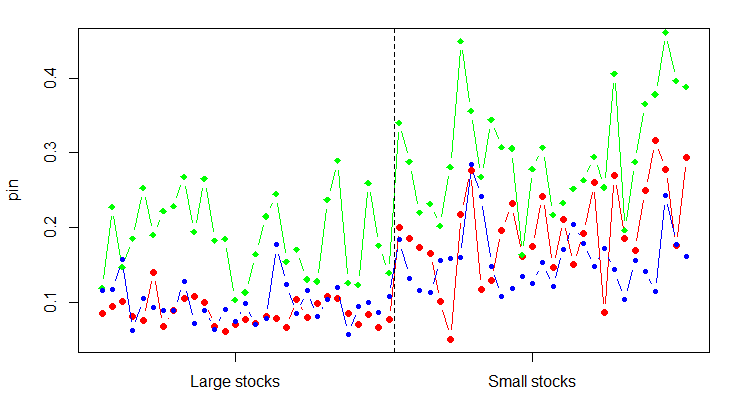
\includegraphics[width=\linewidth]{images/app1-pin_small_large_stocks.png}}%
\subcaptionbox{Alpha for large and small stocks\label{subfig:alpha_levels}}
[.5\textwidth]{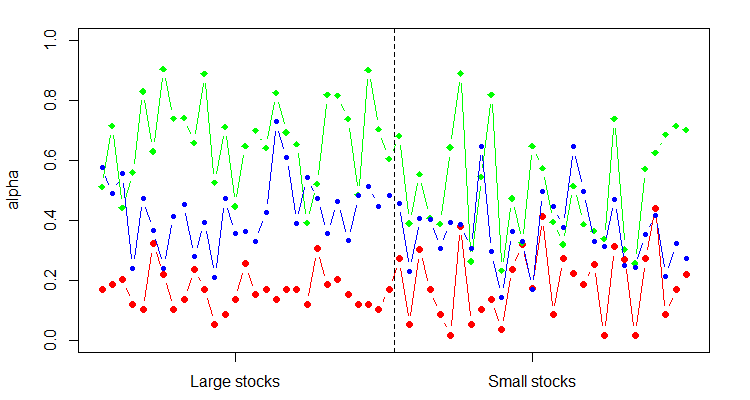
\includegraphics[width=\linewidth]{images/app1-alpha_small_large_stocks.png}}
\caption{Stock-level model comparisons for PIN and Alpha for the different models: PIN (red), MPIN (green), ADJPIN (blue)}
\label{fig:large_vs_small_stocks}
\end{widefigure}

 Figure \ref{subfig:pin_levels} also shows relatively higher estimates in the right side of the panel (small stocks), as well as high stock-based variations, e.g., for the MPIN model PIN estimates range from 10$\%$ to around 40$\%$ for the examined stocks. 
 Figure \ref{subfig:alpha_levels} replicates Figure \ref{subfig:pin_levels} for alpha parameter estimates (information event occurrence probability).  It shows that PIN model consistently has lower alpha estimates than MPIN and ADJPIN models, but with higher variability, ranging from 2\% to 42\%. Significant differences in alpha estimates are observed among the three models and across stocks. Therefore, a careful analysis of each model's assumptions is necessary to draw any conclusions.

\subsection{Example 2 – VPIN and announcements}

Using over 5.4 million trades on 58 Swedish stocks spanning 59 trading days during the last quarter of 2020, we estimate VPIN with three different parameter sets, i.e., \code{1-50-50}, \code{1-1-5}, and \code{5-1-5} \footnote{The first parameter set \code{1-50-50} is the main setting used in several studies \citep[see e.g.][]{Easley2011microstructure, Easley2012Flow, Abad2012From}. The parameter sets \code{1-1-5}, and \code{5-1-5} are two of the several sets previously used for comparative purposes \citep[see e.g.][]{Abad2012From}.}.

In each parameter set \samp{a-b-c}, \code{a} represents the length of time bars in minutes, \code{b} stands for the number of buckets per a day with average trading volume, \code{c} is the number of previous buckets used in the calculation of VPIN at any bucket. In line with \cite{Easley2011microstructure,Easley2012Flow}, we select the  parameter set \code{1-50-50} as our main setting.

Table \ref{tab:desc_statistics_vpin_measures} presents the summary statistics for VPIN estimates for the three settings, and this for both the whole sample, and for the large and small stocks separately. 
Mean (median) VPIN with \code{1-50-50} is \( 27.6\%\) (\( 25.3\%\)) for the whole sample. Number of VPIN observations is \(166,875\), almost equally composed of observations on small and large cap stocks. Mean VPIN is slightly larger for the small stocks (\(28.1\%\) and \(27.2\%\), respectively). 



\begin{table}[ht]
\caption{Descriptive statistics for three settings of VPIN - for large, small, and all stocks.}
\label{tab:desc_statistics_vpin_measures}
\renewcommand{\arraystretch}{1.15}
\setlength{\arrayrulewidth}{1pt}
\small
\setlength{\tabcolsep}{1.5pt}
\begin{tabular}{p{1.4cm} p{1.2cm} p{1.3cm} p{1.3cm} p{1.3cm} p{1.3cm} p{1.3cm} p{1.3cm} p{1.3cm} p{1.3cm} }
\toprule
\multicolumn{10}{p{14cm}}{\footnotesize N refers to the number of observations; min and max refer to the minimum, and maximum values respectively. SD corresponds to the standard deviation, while Qx is the x\textsuperscript{th} quantile.}\\
\midrule
\textbf{Setting} & \textbf{Sample} & \textbf{N} & \textbf{mean} & \textbf{min} & \textbf{Q25} & \textbf{Q50} & \textbf{Q75} & \textbf{max} & \textbf{SD}
\\ \hline
        \code{1-50-50} & \code{Large} & 84131 & 27.2 & 10.7 & 21.4 & 25.1 & 30 & 92.9 & 9.2 \\ 
        \code{1-50-50} & \code{Small} & 82744 & 28.1 & 0 & 14.1 & 25.8 & 39 & 100 & 18.2 \\ 
        \code{1-50-50} & \code{All} & 166875 & 27.6 & 0 & 19.5 & 25.3 & 33.6 & 100 & 14.4 \\ 
        \code{1-1-5} & \code{Large} & 1595 & 6.9 & 1.2 & 4.7 & 6.3 & 8.5 & 22.8 & 3.1 \\ 
        \code{1-1-5} & \code{Small} & 1568 & 13.5 & 0.7 & 8.2 & 12.5 & 17.1 & 62.5 & 7.5 \\ 
        \code{1-1-5} & \code{All} & 3163 & 10.1 & 0.7 & 5.6 & 8.3 & 13 & 62.5 & 6.6 \\ 
        \code{5-1-5} & \code{Large} & 1595 & 9 & 1.2 & 6.2 & 8.2 & 10.6 & 33.2 & 4.3 \\ 
        \code{5-1-5} & \code{Small} & 1568 & 18.3 & 0.6 & 11.3 & 16.2 & 23.2 & 89.1 & 10.3 \\ 
        \code{5-1-5} & \code{All} & 3163 & 13.6 & 0.6 & 7.5 & 10.8 & 17.2 & 89.1 & 9.1 \\ 
\bottomrule
\end{tabular}
\end{table}

Under the basic setting, the difference between mean VPIN measures of small and large stocks, while in line with our expectations, it is not as large as previous studies suggest. For instance, \cite{Abad2012From} report mean VPIN values of \(25\%\) and \(53\%\) for the Spanish large and small stocks, respectively. We too obtain positive difference between the mean VPIN values for small and large stocks for all parameter sets. The VPIN value for small stocks is substantially larger than for large stocks (almost twofold) for settings, for which an average trading day contains a single bucket, and five buckets are used in calculating the VPIN (parameter sets \code{1-1-5} and \code{5-1-5}). The excess informed trading of small stocks is not restricted to average values. For instance, under our basic setting, first and third quartiles of VPIN for the whole sample are around \(20\%\) and \(34\%\). This range as well as the standard deviation for small stocks are relatively larger than those of large stocks.

We turn now to investigate whether the correlation observed between the VPIN distribution and the absolute post returns distribution for the S$\&$P 500 E-mini index, as reported by  \cite{Easley2011microstructure},  can be generalized to (1) individual stocks, (2) another (non-US) market, i.e. NASDAQ Stockholm, (3) more recent data, (4) positive and negative post-returns. To do this, we replicate the two tables (Exhibit 7 and 8) as they appear in  \cite{Easley2011microstructure} for individual stocks, for absolute post-returns initially, before differentiating between positive and negative post-returns. Table \ref{tab:table_distributions_vpin_absolutereturns} reports, in Panel A, the distribution of the absolute post-returns conditional on VPIN. Each of the 3 rows represents the distribution in percentage for the \(0-5^{th}\), \(45^{th}-50^{th}\), 
\(95^{th}-100^{th}\) quantiles of the VPIN values. Respective quantile values are given in the first column (e.g., \(0.062\) is the $5^{th}$ quantile of VPINs in our data). % The values in each row add up to \( 100\). 


The results in Table \ref{tab:table_distributions_vpin_absolutereturns} (Panel A) are significantly similar to the results in  \cite{Easley2011microstructure}, both qualitatively, and even quantitatively. For instance, the share of large absolute post-returns is highest in the highest VPIN quantile, and substantially higher than the same share in other quantiles. The share of large absolute post-returns (exceeding \(2\%\)) associated with the highest VPIN quantile is \(2.16\%\), while it is below \(0.44\%\) for the $45^{th}$ to $50^{th}$ VPIN quantiles. The highest levels of VPIN (in the highest quantile) have \(4.5\) times higher likelihood to be followed by large absolute post-returns than intermediate levels of VPIN (in the median quantile) $(2.16\%$ and $0.44\%)$. This ratio is strikingly similar to the one found in the referenced paper $(0.22\%$ and $0.05\%)$. 
However, the likelihood of large absolute post-returns is higher in our study $(2.16\%$ vs $0.22\%)$, which is likely due to our use of individual stocks rather than an index. 
For each of the absolute return intervals larger than 0.5$\%$, the share of VPIN values in the highest quantile is at least twice as large as the ones in lower quantiles. The share of VPINs within the highest quantile (last row of Table \ref{tab:table_distributions_vpin_absolutereturns} - Panel B) is noteworthy: Absolute returns larger than 1$\%$ are highly likely to be preceded by a high VPIN value. In our unreported results, for over 40$\%$ of intraday periods with absolute returns larger than 2\%, the (preceding) VPIN is at its highest quantile.

\begin{table}[H]
\caption{Conditional distributions of VPIN and absolute post-returns}
\label{tab:table_distributions_vpin_absolutereturns}
\renewcommand{\arraystretch}{1.15}
\setlength{\tabcolsep}{3pt}
\setlength{\arrayrulewidth}{1pt}
\small
\begin{tabular}{p{1.2cm}p{1.2cm}p{1.2cm}p{1.2cm}p{1.2cm}p{1.2cm}p{1.2cm}p{1.2cm}p{1.2cm}p{1.2cm}}
\toprule
\multicolumn{10}{p{14cm}}{\footnotesize Panel A provides the distribution of absolute post returns (leading VPIN bucket return) conditional on VPIN values, while Panel B provides the distribution of VPIN values conditional on the absolute post returns. For brevity, only the $5^{th}$, $50^{th}$ and $100^{th}$ quantiles are reported in each panel. Numbers are given in percentages.}\\
\midrule
\multicolumn{10}{p{14cm}}{\textbf{Panel A: Absolute post-returns conditional on VPIN}}\\
\midrule
&  0.25&  0.5&  0.75&  1&  1.25&  1.5&  1.75&  2&  >2.00\\
0.062&80.67&10.1&4.68&2.33&0.97&0.53&0.2&0.2&0.32\\
0.253&80.65&13.11&3.15&1.14&0.71&0.43&0.25&0.12&0.44\\
1&74.94&10.09&5.03&2.7&1.82&1.5&1.08&0.68&2.16\\

\midrule
\multicolumn{10}{p{14cm}}{\textbf{Panel B: VPIN conditional on absolute post-returns}}\\
\midrule
&  0.25&  0.5&  0.75&  1&  1.25&  1.5&  1.75&  2&  >2.00\\
0.062&5.19&3.83&5.54&6.21&4.82&4.11&2.62&4.06&2.28\\
0.253&5.19&4.97&3.74&3.04&3.51&3.36&3.24&2.39&3.12\\
1&4.82&3.83&5.97&7.2&9.05&11.68&13.87&13.6&15.19\\
\bottomrule
\end{tabular}
\end{table}


 We now turn to investigate whether the distribution patterns for absolute returns hold true when returns are split into positive and negative and analyzed separately. Table S8 summarizes the results across four panels showing only the lowest, median, and highest $5^{th}$ VPIN quantiles.  
The distribution patterns of preceding VPINs remain consistent for positive and negative returns, except for the return interval $(-0.5\%,0.5\%)$. When VPIN values are within the highest quantile and post return is positive (negative), the likelihood of return in the next volume bucket exceeding $2\%$ $(-2\%)$ is as high as $3.87\%$ 
$(4.31\%)$. These probabilities are more than seven times that of the median quantile. Note that we excluded zero-return observations before analyzing positive and negative returns separately. This might explain why the findings in Table S8 are  more pronounced than those in Table \ref{tab:table_distributions_vpin_absolutereturns}.

Finally, we investigate VPIN around firm-specific announcements. Using 96 firm-specific announcements taking place within the last quarter of \(2020\), and pertaining to the selected stocks, we investigate whether VPIN values change prior to, and following the announcements, and whether the behavior of VPIN around announcements is similar for the large and smalls stocks. Figure \ref{tab:vpin_values_around_announcements} plot the mean VPIN for the \(\left(-100, +100\right)\) volume buckets where \(0\) refers to the announcement bucket, i.e., the bucket, during which the announcement took place. It  represents VPIN values around announcements for the whole sample, and for both large, and small stocks separately. 
The main finding of our analysis on the whole sample is that, mean VPIN starts to increase shortly prior to announcements, and continues to increase post-announcement, reaches a maximum, before starting to decrease to pre-announcement levels.

As shown in Figure \ref{subfig:whole_sample}, mean VPIN starts to increase at bucket $(-13)$ from a level $25.7\%$, monotonically increases for around $50$ buckets, reaching a level of $30.81\%$, before reverting gradually to around its pre-announcement levels.  Mean VPIN of small stocks, in Figure \ref{subfig:large_small}, starts rising at bucket $(-13)$ from a level of $25.6\%$,  and keeps increasing until bucket $(+29)$ reaching a level of $32.4\%$ before starting to gradually decrease. It, then, reaches its lowest post-announcement level at bucket $(+81)$, before starting to rise again.  As for large stocks in Figure \ref{subfig:large_small}, mean VPIN starts rising at bucket $(-7)$ from a level of $25.2\%$, and keep increasing until reaching a level of $30.3\%$ at bucket $(+50)$, before gradually decreasing afterwards.

\begin{widefigure}[H]
    \centering
    \subcaptionbox{Whole sample of stocks\label{subfig:whole_sample}}
[.48\textwidth]{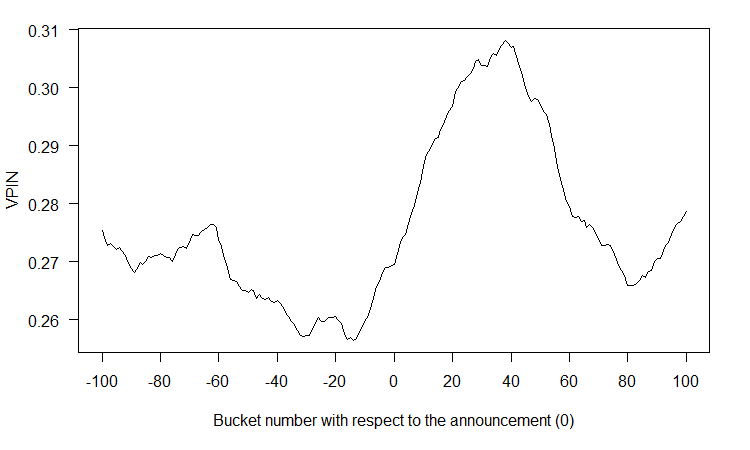
\includegraphics[width=\linewidth]{images/app2-bucket_announcement_pl1.png}}%
\subcaptionbox{Large and small stocks\label{subfig:large_small}}
[.48\textwidth]{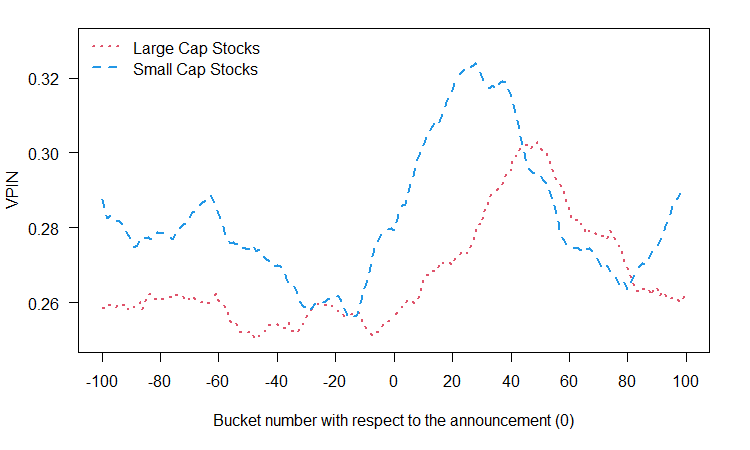
\includegraphics[width=\linewidth]{images/app2-bucket_announcement_pl2.png}}
\caption{Average VPIN around announcements for small, large, and all stocks}
\label{tab:vpin_values_around_announcements}
\end{widefigure}


Interestingly, VPIN starts to react relatively earlier for small stocks than for large stocks. Nevertheless, the presence of early warning property of VPIN is evident for both small and large Swedish stocks. This corroborates with the findings of \cite{Easley2011microstructure, Easley2012Flow}, where they suggest VPIN as a metric providing an early warning signal for intraday events, such as crashes. \cite{Bjursell2017VPIN}  document an increase in VPIN prior to news events, and price jumps in the crude oil market. Similarly, \cite{Bugeja2015microstructure} examining takeover announcements in the Australian markets, find out that VPIN significantly increases for target firms in the four days prior to the takeover announcements.
Our findings suggest the potential of VPIN as an early warning signal might well extend to regular firm-specific events. These VPIN patterns could be further investigated, in light of recent findings on price discovery around announcements in today's financial markets with large HFT prevalence \citep{beschwitz2020first, Ersan2021speed}. 


\section{Conclusion}

\pkg{PINstimation} is an attempt to centralize, and implement in a rigorous manner, the main estimation methods suggested in the literature.  In addition to efficiency, we aim that \pkg{PINstimation} be (1) all-encompassing, i.e. it includes the main model treating the probability of informed trading and its most relevant extensions, (2) complete, i.e it includes not only the tools required to estimate PIN models, but also algorithms to generate initial parameter sets, tools to simulate datasets, and algorithms to aggregate high-frequency trades into daily trading data, and (3) up-to-date, as the current version of \pkg{PINstimation} package is highly up to date including several methods suggested in 2020-2022. 

Future work on the package aims at continuous extension of the package with the most up-to-date estimation methods available. For instance, we have recently added function \code{pin\_bayes()} which implements a Bayesian approach for the estimation of the original PIN model as suggested by \cite{griffin2021}. Even though the \pkg{PINstimation} package aims to be all-encompassing, it remains primarily dedicated to the estimation of probability of informed trading (PIN) models. Thus, other informed trading measures suggested in the literature are, and shall remain, beyond the scope of the package. By the introduction of the package, we hope to contribute to widen the user base of PIN models both in academic circles, and among practitioners; as well as improve the validity, and the comparability of scientific findings within the field.



\hypertarget{refs}{}

\bibliography{pinstimation.bib}

\address{%
Montasser Ghachem\\
Department of Economics, Stockholm University\\%
Stockholm, 106 91, Sweden\\ Sweden\\ (0000-0001-6991-3316)\\
%
%
%
\href{mailto:montassar.ghachem@su.se}{\nolinkurl{montassar.ghachem@su.se}}%
}

\address{%
Oguz Ersan\\
International Trade and Finance Department, Kadir Has University\\%
Istanbul, 34083\\ Turkey\\ (0000-0003-3135-5317)\\
%
%
%
\href{mailto:oguzersan@khas.edu.tr}{\nolinkurl{oguzersan@khas.edu.tr}}%
}
